\RequirePackage{luatex85,shellesc}
\documentclass[]{resonance}
\usepackage{pgf,tikz}
\usepackage{tikzsymbols}
\usepackage[breakable]{tcolorbox}
\usepackage{nameref}
\usepackage{pgfplots}
\usepackage{grffile}
\usepackage{amsmath}
\usepackage{lipsum}  % remove after testing.
\usepackage{mathtools}
\usepackage{wrapfig}
\usepackage{chemfig}
\usepackage{siunitx}
\usepackage{todonotes}
\usepackage{tabularx} 
\usepackage{amssymb}
\usetikzlibrary{shapes,backgrounds,calc,arrows,arrows.meta}

\usepackage[acronym]{glossaries}
%\newglossaryentry{CaM}
%{
%    name=Calmodulin,
%    description={Calmodulin}
%}

\newacronym{camkii}{CaMKII}{calcium/calmodulin dependant protein Kinase II}
\newacronym{cam}{CaM}{calmodulin}
\newacronym{psd}{PSD}{Post Synaptic Densitiy}
\newacronym{ca}{Ca\textsuperscript{++}}{calcium}
\newacronym{pp1}{PP1}{protein phophatase 1}
\newacronym{pp2}{PP2}{protein phophatase 2}
\newacronym{cacam}{Ca\textsuperscript{++}/CaM}{calcium/calmodulin complex}
\newacronym{i1p}{I1P}{phosphorylated inhibitor-1}
\newacronym{i1ppp1}{I1P.PP1}{I1P-PP1 complex}
\newacronym{i1}{I1}{inhibitor-1}
\newacronym{can}{CaN}{calcineurin}
\newacronym{pka}{PKA}{protein kinase A}
\newacronym{darpp}{DARPP-32}{a dopamine- and cyclic-AMP regulated neuronal phosphoprotein}
\newacronym{i2}{I2}{inhibitor 2}
\newacronym{sbgn}{SBGN}{System Biology Graphical Notation}
\newacronym{ltp}{LTP}{Long Term Potentiation}
\newacronym{ltd}{LTD}{Long Term Depression}
\newacronym{nmda}{NMDA}{N-methyl-D-asparate}
\newacronym{nmdar}{NMDAR}{N-methyl-D-asparate receptor}
\newacronym{ampa}{AMPA}{$\alpha$-amino-3-hydroxy-5-methyl-4-isoxazolepropionic acid}
\newacronym{mz}{MZ}{Miller and Zhabotinksy}


\newcommand\Fig[1]{\textit{Figure~\ref{#1}}}
\newcommand\TT[1]{\texttt{#1}}

% Title Page
\title{Switches in the brain?} 
\secondTitle{A potential mechanism for long-term memory storage}
\author{Dilawar Singh}
\date{\today}
\begin{document}
\maketitle

% Author info here
\authorIntro{
    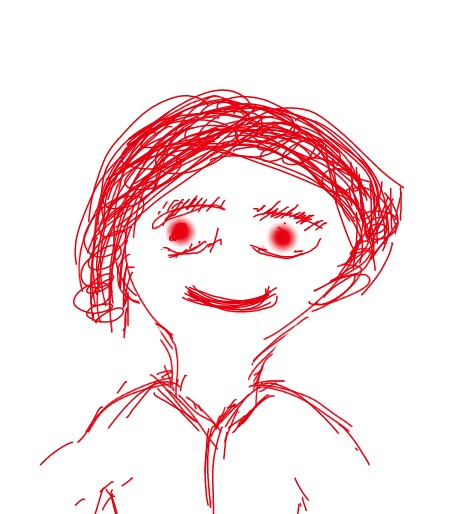
\includegraphics[width=2cm]{./dilawar.jpg}\\
    Dilawar Singh is currently a graduate student at National Center for
    Biological Sciences (NCBS), Bengaluru. His hobby is to convince people to
    move to open-source softwares to live happily ever after.
}


\begin{abstract}

    We forget often. But we remember some memories as long as we live.
    This means that our brain is capable of protecting memories for years.
    This is a remarkable feat given that the \emph{biochemical hardware}
    involved in creating new memories is a hostile place for
    its storage.  What are the challenges involved? And what type of 
    biochemical mechanisms may overcome them? This article explores a major
    hypothesis that molecular switches may be behind our remarkable ability to
    remember for a lifetime.

\end{abstract}

\maketitle
\monthyear{May 2018}
\artNature{GENERAL  ARTICLE}

\section{Introduction}\label{sec:intro}

Our brain is made up of roughly 100 billion neurons, joined together with over
100 trillion connections called \textbf{synpase}s. Each neuron on average makes
1000 connections. It is now widely accepted that memories are created by
changing these connections. 

Let's label these synapses as $s_1, s_2, \ldots s_n$. A subset of these synapses
participate in a specific memory formation. For example, my memory of being
chased by a ferocious street dog named \emph{Lalu} (lets call it
$M_\text{Lalu}$) is represented by the set of the synapses
$M_\text{Lalu}=(s_{10}, s_{21}, s_{12},\ldots,s_{331})$ i.e. these connections
were changed during my troubling encounter with Lalu. I sometimes recall this
memory whenever I see a similar looking dog. 

%% The ability to learn quickly from an experience and to recall it has obvious
%% advantages. Learning is a form of memory (and so is confidence). We are going to
%% use these terms interchangeably. The ability to remember and recall painful
%% encounters with predators helps all animals in avoiding them.  The ability to
%% remember the location or cue of food, water and mates, seasonal events for
%% migration or reproduction are just a few other examples of usefulness of memory. 

\begin{figure}[!b] 
    \caption{Memory formation and forgetting. During formation of
    a memory, some synapses become stronger. The longer you can maintain these
    connections, the longer you can hold on to this memory.}
   \label{fig:engram}
   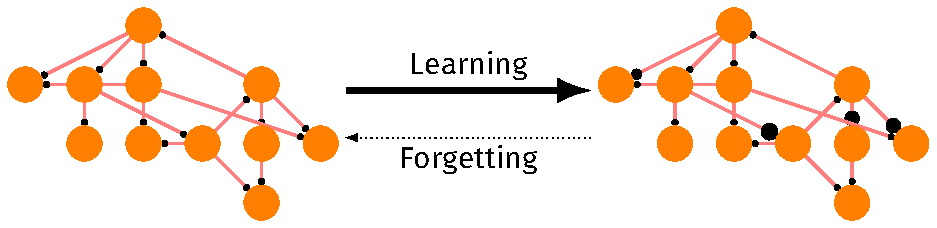
\includegraphics[width=\linewidth]{engram.pdf} 
\end{figure}

I can recall an experience as long as the set of synapses in which the
particular experience was stored remains \emph{intact}. Therefore our
ability to remember is contingent on our brain's ability to keep its connections
intact.  But on the other hand, our ability to learn is depends on our brain's
ability to change its connections. And here is the first challenge!

\subsection{Learning quickly v/s forgetting slowly, a zero-sum game}\label{subsec:zero_sum} 
\leftHighlight{
    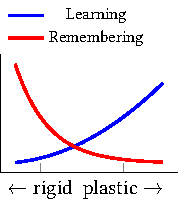
\includegraphics[]{./foget_remember.pdf}
    Ability to change (plasticity) is good for learning, but bad for remembering.
}

For $M_\text{Lalu}$ (or any other memory) to remain intact, each of its
component ($s_{10}, s_{21}, s_{12} \ldots$) should also remain intact.  The
longer a synapse can keep itself unchanged, the better it will be at keeping the
memory. Lets assume that somehow I create a synapse which maintain its state for
a very long time (i.e. a rigid synapse). This synapse will not \emph{forget}
easily, but it causes another problem. Rigid synapse will not participate in any
memory formation anymore since learning requires change and it can't change. It
behaves like a read-only compact disk. On the other hand, if I create a synapse
which is easily changeable (i.e. a plastic synaspe), it will be good at learning
new experiences but won't be able to retain it for long. Plastic synapse forgets
easily.  We know that not only we remember for long time, we are capable of
learning quickly too. For example, honey bees can learn the location of food
after one encounter with flowers.  Indeed a good memory system is the one which
learns quickly from new experiences and forgets old information as slowly as
possible.  Forgetting and remembering are the two sides of the same coin.  They
are conflicting demands -- a zero-sum game.  The challenge is to strike a
balance. 

% Hopefield network 
\section{Hopfield network -- associative memory network}\label{sec:hopfield}

% \begin{quote}
% In mathematical networks, synaptic plasticity is the only non-trivial element 
% available to produce interesting behaviour. If model networks can achieve anything 
% approaching the behaviour of their biological counterparts then it will be clear 
% that synaptic plasticity is remarkably powerful and likely to be of crucial importance. 
% On the other hand, if the mathematical models cannot approach biological complexity then 
% other elements such as more accurate descriptions of individual cell behaviour will 
% have to be included in the models until we learn what minimum set of behaviours is needed 
% to mimic biological systems. \\
% \hfill -- L F Abbott
% \end{quote}

% Before we continue further, lets familiarize ourselves with one very popular
% network which is made up of neuron like elements. In this network, patterns can
% be stored and recalled.

Memory storage and retrieval is trivially done by a computer. It will be helpful
to compare memory storage in the computer and the brain. In the computer, we
always know the address of every stored memory and we access it by providing
this address. The file icon on your desktop is a graphical way of encoding this
addressing scheme. This process is very similar to looking up the index page in
a reference book to find a chapter. Our brain, on the other hand, is very
unlikely to have such an indexing mechanism. 

We recall when we are provided with \textit{cues}. For example, when you see
some part of of a familiar person in a wedding album -- while the rest of the
person may be hidden behind others -- you could easily identify the person. And
many other memories of that person will also be recalled. A famous class of
recurrent neural network popularly known as Hopefield network can do just the
same as shown in \Fig{fig:hopfield}.

\begin{figure}[!hb]
    \centering
    \caption{Hopfield network with 100 spiking neurons. These \emph{recurrent} 
        configurations give rise to interesting brain-like
        computation. \textbf{(B)} 6 patterns (memory) i.e. NCBSXY are stored in this
        network. \textbf{(C)} When a very distorted \textit{cue} is applied to
        the network input, it \textit{fetches} one of stored pattern which is
        the \emph{closest} to the applied cue.
    }\label{fig:hopfield}
    \includegraphics[width=\linewidth]{./hopfield.pdf}
\end{figure}

How does this recurrent network work is beyond the scope of article. Readers are
encouraged to explore more by themselves. \emph{``How well we can explain biological
memory by these network''} is an active research area.  Though these networks are
extremely successful in accomplishing various \textit{brain-like} computation
(\textit{a la} machine learning), I would like to advise the reader to be sceptical by
noting the following:

\begin{itemize}
    \item  Neurons used in these networks are highly simplified. \textit{Real}
        neurons are not this simple. Even though these simplified neurons
        capture the essential \textit{all-or-none} (electrical spike) way of
        communication and learning by changing synaptic connections, they do
        ignore rich local computations which can be accomplished by branches of
        these neurons called \textit{dendrites}.
    \item  There is no strong evidence that neurons make such dense recurrent
        connections. However some studies have shown that Hopfield network can
        work with very sparse recurrent connections as well. 
    \item Activity in these networks does not match usually observed activity 
        in the primate brain during memory-recall experiments.
\end{itemize}

\leftHighlight{Solutions contributed by other disciplines are helpful for
comparison and contrast and often provide very useful insight. But in the end, these
solutions must be tested under the constraints imposed by biology.}

Nonetheless, these network provide us with a framework to concretely think about
the problem of memory storage and its recall. We learn a great deal about these
problem by pointing out the limitations and failure of these models. Hopfield
network has properties which will sound very natural to us. Can you store as
many memories as you like in these networks? No. There is an upper limit. Adding
more patterns over maximum limit causes distortion in memories. When a cue is
given, the network no longer fetch the right pattern. It often fetches a pattern
which was not even stored; the retrieved pattern instead resemble some mixture
of many stored patterns. When too many memories are stored, they corrupt each
other by mixing up. One can ask more questions. What if connections are allowed 
to decay in these networks, and when memories starts disappearing, do the
weakest memory disappearing first or the newest? When a new memory is added,
what do happen to the old memories?

After this necessary detour, lets go back to the main theme: how do synapses
maintain their state?

\section{How does a synapse maintain its state?}

Very complex biochemistry plays out during learning that changes the synapse.
Surprisingly, the net effect of this complex biochemistry can be summarised by a simple
mathematical expression. Ah, \emph{the unreasonable effectiveness of
mathematics}\cite{unreasonable_math}! Let's assume that synaptic strength $w$ is
tightly correlated with a chemical species $X$ found at synapse i.e. $w$ changes
with $X$.  The problem of maintenance of $w$ can be rephrased as the problem of
maintenance of the level -- or the activity -- of $X$. Therefore, the problem of
``\emph{synapse maintaining its state}'' becomes the problem of ``molecule
\emph{$X$ maintaining its state}'' -- a more concretely defined problem.

\begin{figure}[h!]
    \caption{Phosphorylation and deposphorylation of X. P is phosphatase.}\label{fig:model}
    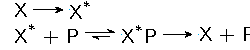
\includegraphics[]{./fig_model.pdf}
\end{figure}

Lets assume that $X$ is converted to its \texttt{ACTIVE} form $X^*$  by adding a
phosphoryl group ($PO_4^{2-}$). The phosphoryl group is removed by a phosphatase
and $X^*$ is turned back into \texttt{INACTIVE} $X$. The phosphorylation and its
counterpart dephosphorylation are a very common motif for controlling various
chemical reactions by \textit{activating} and \textit{inactivating} protein
molecules. Once most if not all $X$ has been turned into $X^*$ during
memory formation, how do we make sure that $X^*$ does not turn back into $X$
(lose memory)?

\rightHighlight{Can you think of other set of hypotheses? It must conform to laws of chemistry!}
Let's mull over a solution to this problem of long term maintenance of $X^*$.
Let's assume that somehow followings are true. 
\begin{enumerate}
    \item \textbf{(Amplification)} $X^*$ \textbf{auto-phosphorylate} itself i.e. \tikz[baseline]{ 
            \node (x) {$X$};
            \node[right=9mm of x] (xp) {$X^*$};
            \draw[-latex] (x) -- (xp);
            \draw[-latex] (xp) edge[out=120, in=90] ([xshift=7mm]x);
        }. If we manage to get sufficient $X^*$ somehow, it
        will act as a catalyst to its own production. $X^*$ will always remain
        high.
    \item Dephosphorylation of $X^*$ is minimized by controlling the number of
        $P$ or reducing the reaction rate.
\end{enumerate} 

Both (1) and (2) help in making $X^*$ highly stable. Problem solved? No.  Now
we have constructed a rigid synapse. Recall the \textit{rigid} v/s
\textit{pastic} synpase dilemma discussed previously (section
\ref{subsec:zero_sum}). This synapse will definitely remember for longer
but it will not participate in any new learning anymore.

As long as we are in the realm of theory, let's propose a solution to this
problem . We add another reaction say $P'+X^*\rightarrow P'X \rightarrow P'+X$
which deactivates $X^*$ when the \textit{need} arise. Phosphatase P' is different
than P. This adds another layer of control to an already complicated problem i.e.
forgetting is now controlled by another process. This requires one more
explanation: how does this new mechanism controlling \textit{forgetting} works?
And philosophically -- if you care about it -- it violates the principle of
\textbf{parsimony} which recommends to pick the simplest explanation.

We still have two big problems hiding underneath. We have not considered the
underlying biological hardware i.e. synapse in any detail where this biochemical
network suppose to function. The first problem is chemical noise 
. For biochemical system operating in very small volumes,
effect of chemical noise can be very strong. \leftHighlight{The volume of a
typical synapse is \SI{1e-20}{\cubic\meter}. At this volume, \SI{1}{\micro M}
concentration is roughly equal to 6 molecules.} There are over 200 types of
protein molecules in a typical synapse. Indeed, most of these protein molecules have few
tens of molecules.  The brain is always active and  the chemical noise caused by
the background activity in the brain will surely turn some molecules of $X$ into
$X^*$. Then due to auto-phosphorylation, sooner than later, all of the $X$ will be turned
into $X^*$. We have created a very stable memory of nothing but background
noise. This is highly undesirable!

The second problem is \textit{turnover} i.e. old molecules are constantly degraded
and being replaced by newly minted molecules. Assume that at the time of memory
formation, we had 100 molecules of $X^*$ in synapse. And also assume that on
average, every day one new molecule (i.e. $X$) replaces an old one ($X^*$).
After 50 days, half of the synaptic strength is gone! We must have a
\textit{refresh} mechanism by which we make sure that the new molecule quickly
changes its state according to the state of synapse i.e. newborn $X$ becomes
$X^*$ most molecules at synapse are $X^*$.

Effectively, we want a stable \texttt{ACTIVE} state (where all $X$ are $X^*$)
and don't want chemical noise to turn $X$ into $X^*$. We want a switch like
behaviour -- if it is \textit{OFF} or \text{ON} it tends to stay \textit{OFF} or
\texttt{ON} respectively. A significant force is required to flip a switch; it
does not get flipped by noise. If few $X$ are turned into $X^*$ by background
noise, we expect them to be quickly turned back into $X$ by phosphatase. And if
during memory formation, a significant portion of $X$ has been turned into $X^*$
then we expect that any $X^*$ turned back into $X$ is quickly activated again
into $X^*$.  This system should operate like a switch which does not flip unless
significant force is applied. These are called \textbf{bistable switch}es. 

\begin{figure}[t!]
\centering
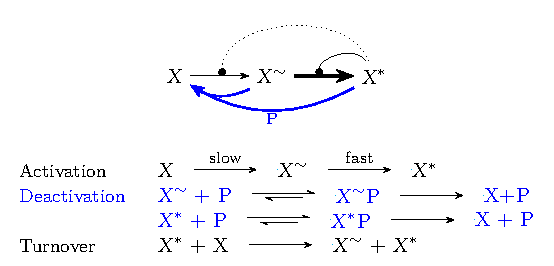
\includegraphics[width=\linewidth]{./fig_model_b.pdf}
\caption{A hypothetical network which can solve the problem of chemical noise and
    turnover with suitable parameters (how?). The activation step is divided into slow and fast
    components such that fluctuations caused by background noise do not cause system to 
    activate itself. $X^*$ also partially activate $X$ to $X^\sim$ to overcome \textit{turnover}. 
}\label{fig:model_bistable}
\end{figure}

Is there any  proof that bistable systems are even possible? Do they occur at
all in living cells?  Bistability (and its close relative oscillations) are very
common in biology; from cellular level to population levels. So if it won't be
surprising if we find bistable switches in syanpses as well.  \emph{Is there a set
of chemical reactions which forms a bistable switch at synapse?} Various studies
have shown that \gls{camkii} may form a bistable switch in synapse.

\section{Molecular bistable switch at synapse}\label{sec:molecular_switch}

\begin{figure}[ht!]
    \centering
    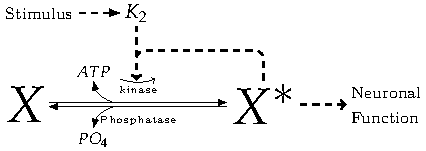
\includegraphics[width=8cm]{./lisman_bistable.pdf}
    \caption{Reaction in a bistable switch proposed by John Lisman. Modified
        from \cite{lisman1985}. Permission not required for reuse for
        educational purpose.
    }\label{fig:lisman}
\end{figure}

John Lisman hypothesised that a kinase and a phosphatase together
(\Fig{fig:lisman}) can form a bistable switch which is stable against
\emph{turnover}. \gls{camkii} and its phosphatase \gls{pp1} were identified as
the hypothesised kinase and phosphatase. This chemical system had been
extensively studied using computational models for over two decades
\cite{sandstorm}. There is evidence that \gls{camkii} is bistable \emph{in
vitro} conditions. 

%\begin{tcolorbox}[
%    title = \bfseries \centering Box \newboxText. \gls{camkii}: A brief overview of its properties and function
%    , breakable
%    % , grow to left by=4cm
%    , text width=13.5cm
%    % , height = \pageheight
%    ]
% CaMKII box.
\boxTextodd{\gls{camkii}: A brief overview of its properties and function} {
Among more than 2000 proteins found in brain, \gls{camkii} constitutes
roughly 2\% of all. Furthermore, it is enriched in Hippocampus -- a brain
structure essential for memory formation. Indeed, \gls{camkii} is known to
play essential role in memory formation.  In experiments involving mice,
deactivating \gls{camkii} in any way has always resulted in impairment of
memory formation and learning. 

\gls{camkii} molecule has many interesting properties which makes it an
attractive candidate for storing memory. 12 to 14 subunits of \gls{camkii} make
up one holoenzyme, usually arranged in dodecameric (top view \tikz{  \foreach \i
in {1,2,...,6} { \node[circle, fill=blue!50, shift=(60*\i:1mm),inner
sep=1pt] (b\i) at (0,0) {}; } }) or tetradecameric form (top view \tikz{
\foreach \i in {1,2,...,7} { \node[circle, fill=blue!50,
shift=(360*\i/7:1mm),inner sep=1pt] (b\i) at (0,0) {}; } }). \gls{camkii}
structure is shown in (\textbf{A}) below (from Protein Data Bank
(https://www.rcbs.org)).

\vspace{5mm}
\begin{tabularx}{\linewidth}{p{3cm} X}
\textbf{A}

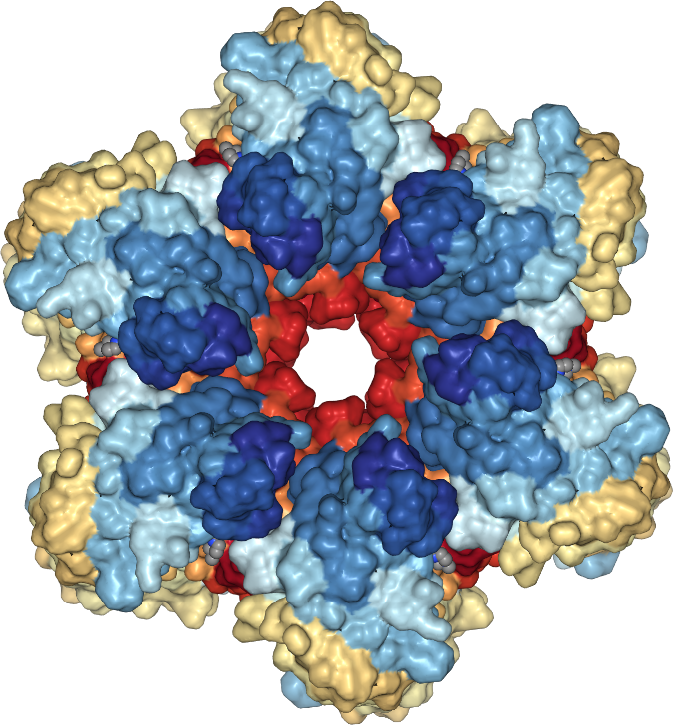
\includegraphics[height=2cm]{./camkii_pdb.png}
&
\textbf{B} 

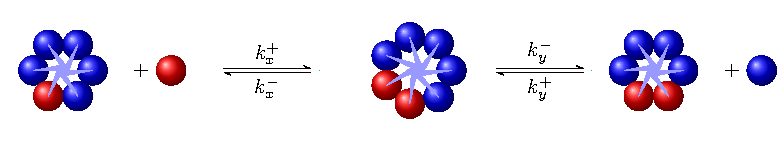
\includegraphics[width=9cm]{./camkii_subunit_exchage.pdf}
\\
\textbf{C} 

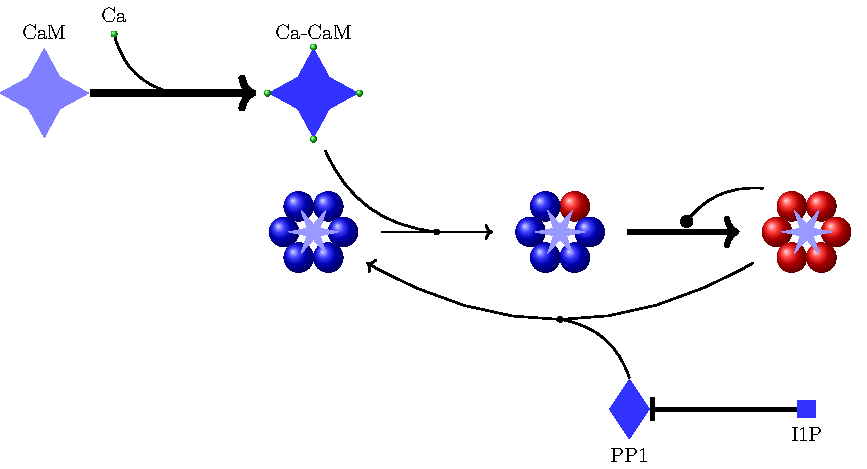
\includegraphics[width=8cm]{./camkii_pp1_switch_level1_detail.pdf}
\end{tabularx}

In \textbf{(B)}, we show subunit-exchange between two holoenzymes i.e. a fully
active \gls{camkii} holoenzyme can loose an \textit{ACTIVE} subunit which can be
picked up by another holoenzyme and it becomes partially active. In
\textbf{(C)}, we summarise the activation pathway of \gls{camkii}. Upon its
influx into synapse, \gls{ca} binds to \gls{cam} and create a complex
\gls{cacam}. \gls{cacam} binds to \gls{camkii} and phosphorylate it. Note that
first step involving activation of its first subunit is very slow for it
requires binding of two \gls{cacam} simultaneously. Once a subunit has been
activated, it helps in activation of its neighbours (only one \gls{cacam} is
required now and therefore further phosphorylation proceeds at much faster
rate). 

Note that the first very slow step of \gls{camkii} phosphorylation can be
overcome by subunit-exchange. If an inactive holoenzyme has picked up an active
subunit via subunit-exchange, it does not require simultaneous binding of two
\gls{cacam} molecules. Therefore subunit exchange helps in spreading
\gls{camkii} activation. It is interesting to note that via subunit exchange,
\gls{camkii} can act at distance even when it is anchored in one place.  

\paragraph{Integration of \gls{ca} signal} A single \gls{camkii} holoenzyme acts
as a leaky integrator of \gls{ca} activity i.e. it sums up \gls{ca} activity in
time and also decays with a time-constant. Effectively it is similar to a leaky
capacitor (\gls{ca} activity is applied current).
} % box ends here.
% \end{tcolorbox}

In our computational study of this pathway, we show that subunit-exchange
improves information retention capacity of \gls{camkii}. We also show that
distributed clusters of \gls{camkii} can form very stable bistable switches. And
it also operate as integrator which is often observed in experiments. In short,
we show the subunit-exchange makes \gls{camkii} molecule better at retaining
information and it is likely that \gls{camkii} is bistable in special
micro-environments. To prove it, one needs to observe single molecule activity
in synapse near surface of synapse which is a very challenging experiment.

\begin{figure}[h!]
    \caption{ \textbf{(A)} Graphical representation of \gls{camkii} signalling
        pathway. \textbf{(B)} This pathway shows bistable behaviour when synapse
        is receiving background activity. One trajectory is shown for system with 
        15 molecules. \textbf{(C)} Stability of synapse increases exponentially
        with number of \gls{camkii} molecules. With $\sim 60$ molecules, switch
        remain stable for roughly $150$ years.
    }\label{fig:camkii_summary}
    \centering
    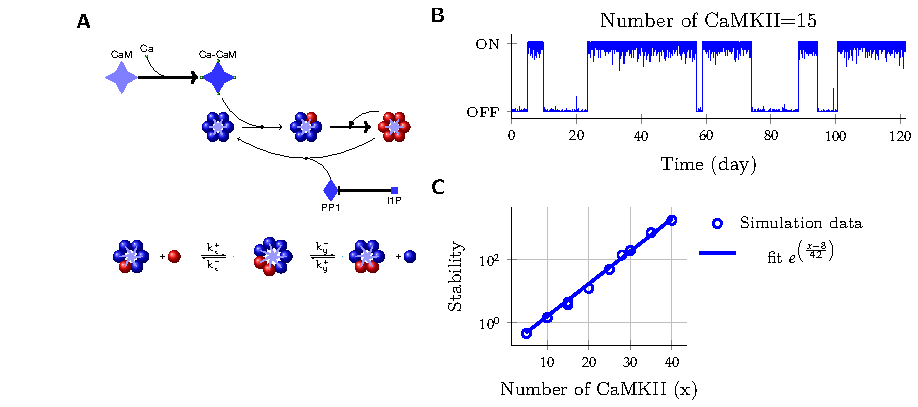
\includegraphics[width=\linewidth]{./resonance_camkii.pdf}
\end{figure}


% References section
\section{Conclusion}

In this article, we have discussed why bistable motif is an attractive candidate
for storing biological memories. Most support for this idea has came from
computational studies. To really prove it, we need experimental data supporting
this hypothesis. There is growing experimental evidence that synapse change in
\textit{all-or-none} manner, a finding which is consistent with this idea. Some
studies claim that changes are graded i.e. synapse changes in step-wise manner
much like a \textbf{multi-stable} synapse. A multi-stable synapse is an ensemble
of many bistable components. Whether \gls{camkii} is bistable in synapse (or in
some part of it) is still an open question. So far there is no concrete evidence
that it is. There could be other still unknown mechanisms which can give rise to
bistability. Given that bistable chemical motifs are widespread, it is
reasonable to believe that there are indeed switches in our brain -- much like
flip-flops in your pen-drives and memory cards -- which are evolved to keep our
memories safe from the onslaught of time and noise.

\section*{Acknowledgements}
I'd like to thank Somya Mani for helpful suggestions on the manuscript.

\correspond{
    Bhalla Lab,
    National Center for Biological Sciences, Bengaluru \\
    GKVK Campus, Bellary Road \\
    Bengaluru - 560065.  \\
    Email: dilawars@ncbs.res.in
}
\begin{thebibliography}{99} 
    \bibitem{lisman1985} 
    Lisman J. E., 
    \textit{A mechanism for memory storage insensitive to molecular turnover: a
    bistable autophosphorylating kinase}. 
    Proc. Natl. Acad. Sci. USA, May 1985

    \bibitem{koch1999}
    Christof Koch
    \textit{Biophysics of computations}.
    Oxford University Press, 1999.

    \bibitem{sandstorm} 
    Malin Sandstorm,
    \textit{Models of CaMKII activation},
    Master Thesis, Royal Institute Of Technology Sweden 

    \bibitem{unreasonable_math}
    Eugene Wigner,
    \textit{The Unreasonable Effectiveness of Mathematics in the Natural Sciences},
     Communications in Pure and Applied Mathematics, vol. 13, No. I (February 1960)

\end{thebibliography}
\end{document}
